%(BEGIN_QUESTION)
% Copyright 2010, Tony R. Kuphaldt, released under the Creative Commons Attribution License (v 1.0)
% This means you may do almost anything with this work of mine, so long as you give me proper credit

Se på dette reguleringssystemet, satt opp for å holde temperaturen i en kjemisk reaktortank på en konstant settpunktverdi. Reaktoren varmes av en dampkappe, der varm damp slippes inn gjennom en motorstyrt (M) reguleringsventil (TV), basert på temperaturen i reaktoren målt av temperatursenderen (TT):

$$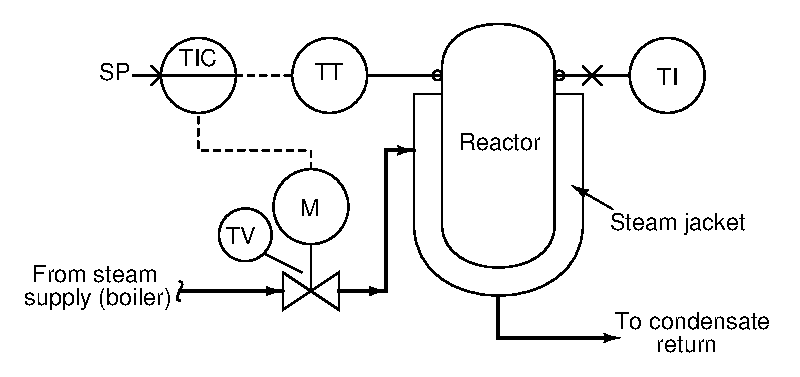
\includegraphics[width=15.5cm]{i00137x01.eps}$$

Du kommer på jobb og finner en svært opprørt operatør. Siste batch fra reaktoren var utenfor spesifikasjon, som om temperaturen var for lav. Likevel viser regulatoren (TIC) temperatur nøyaktig på settpunkt: 175 $^{o}$F.

Første steg er å gå til reaktoren og lese temperaturmåleren (TI) montert ved samme punkt som temperatursenderen. Den viser bare 137 $^{o}$F.

Basert på dette, bestem mest sannsynlig feilkilde og forklar hvordan du kom fram til konklusjonen.

\vskip 20pt \vbox{\hrule \hbox{\strut \vrule{} {\bf Forslag til sokratisk diskusjon} \vrule} \hrule}

\begin{itemize}
\item{} Hvorfor var det en god beslutning å sjekke temperaturmåleren (TI) på reaktoren som første diagnostiske steg?
\item{} En kollega foreslår at problemet kan være feil regulatorvirkning (f.eks. direkte i stedet for revers). Er dette en plausibel forklaring på symptomene her? Hvorfor/hvorfor ikke?
\item{} Kan problemet være at noen lot regulatoren stå i {\it manuell} i stedet for automatisk modus? Forklar hvorfor/hvorfor ikke.
\item{} Ut fra P\&ID-et: er instrumentene pneumatiske eller elektroniske?
\item{} Siden reaktoren er dampoppvarmet: kan vi konkludere at reaksjonen er endoterm (varmeabsorberende) eller eksoterm (varmeavgivende)?
\item{} Sikkerhetsavstengning bruker ofte en «to-av-tre» (2oo3)-algoritme for å velge beste måling fra tre redundante sendere. Forklar hvordan samme prinsipp kan brukes av instrumentteknikeren i feilsøking.
\end{itemize}

\underbar{file i00137}
%(END_QUESTION)





%(BEGIN_ANSWER)

%(END_ANSWER)





%(BEGIN_NOTES)

Problemet ligger mest sannsynlig i temperatursenderen (TT).

\vskip 10pt

Et viktig diagnostisk prinsipp her er {\it to-av-tre}-votering. Ved å sammenligne tre informasjonskilder for samme variabel og bruke flertallsenighet, kan vi bedre finne faktisk verdi selv om utstyr er feil. Teknikeren må avgjøre hvilket instrument som er feil ved å sammenligne tre datapunkter: to instrumenter (visningsregulator og måler) og operatørens vurdering av batchkvalitet. Siden to av tre kilder er enige (batchkvalitet og temperaturmåler), er mest sannsynlig feil i sender/regulatorsløyfen.

Et alternativ er ikke defekt sender, men feilkalibrert prosessvariabelinngang i regulatoren, slik at den viser for høy temperatur selv med korrekt mA-signal fra sender. En annen mulighet er defekt primærelement (RTD, termoelement osv.), som sender feil signal til senderen.





\vskip 20pt \vbox{\hrule \hbox{\strut \vrule{} {\bf Virtuell feilsøking} \vrule} \hrule}

Dette spørsmålet egner seg godt som en «virtuell feilsøking»-øvelse. Når du presenterer diagrammet for studentene, ser du først for deg en bestemt feil i systemet. Deretter presenterer du ett eller flere symptomer på feilen (noe en operatør eller annen bruker kan observere). Studentene foreslår så diagnostiske tester for å finne feiltype og feilsted, som om de var teknikere i feilsøking. Din jobb er å oppgi hvilke resultater disse testene ville gitt, og dokumentere resultatene synlig for alle studentene.

Under og etter øvelsen er det nyttig å stille oppfølgingsspørsmål som:

\begin{itemize}
\item{} Hva forteller resultatet av siste diagnostiske test om feilen?
\item{} Anta at resultatet av siste test var annerledes. Hva ville det da fortalt om feilen?
\item{} Er siste diagnostiske test den beste vi kunne gjort?
\item{} Hva ville vært ideell testrekkefølge for å finne feilen i færrest mulig steg?
\end{itemize}

%INDEX% Basics, control loop troubleshooting: determining cause of control problem
%INDEX% Process: steam-heated reactor vessel (generic)

%(END_NOTES)
